\hypertarget{aco-r_8cpp}{
\section{aco-r.cpp File Reference}
\label{aco-r_8cpp}\index{aco-r.cpp@{aco-r.cpp}}
}
{\tt \#include \char`\"{}Timer.h\char`\"{}}\par
{\tt \#include \char`\"{}Solution.h\char`\"{}}\par
{\tt \#include \char`\"{}Functions.h\char`\"{}}\par
{\tt \#include $<$string$>$}\par
{\tt \#include $<$list$>$}\par
{\tt \#include $<$map$>$}\par
{\tt \#include $<$stdio.h$>$}\par
{\tt \#include $<$stdlib.h$>$}\par
{\tt \#include $<$iostream$>$}\par
{\tt \#include $<$math.h$>$}\par
{\tt \#include $<$ctime$>$}\par
{\tt \#include $<$cstdlib$>$}\par


Include dependency graph for aco-r.cpp:\nopagebreak
\begin{figure}[H]
\begin{center}
\leavevmode
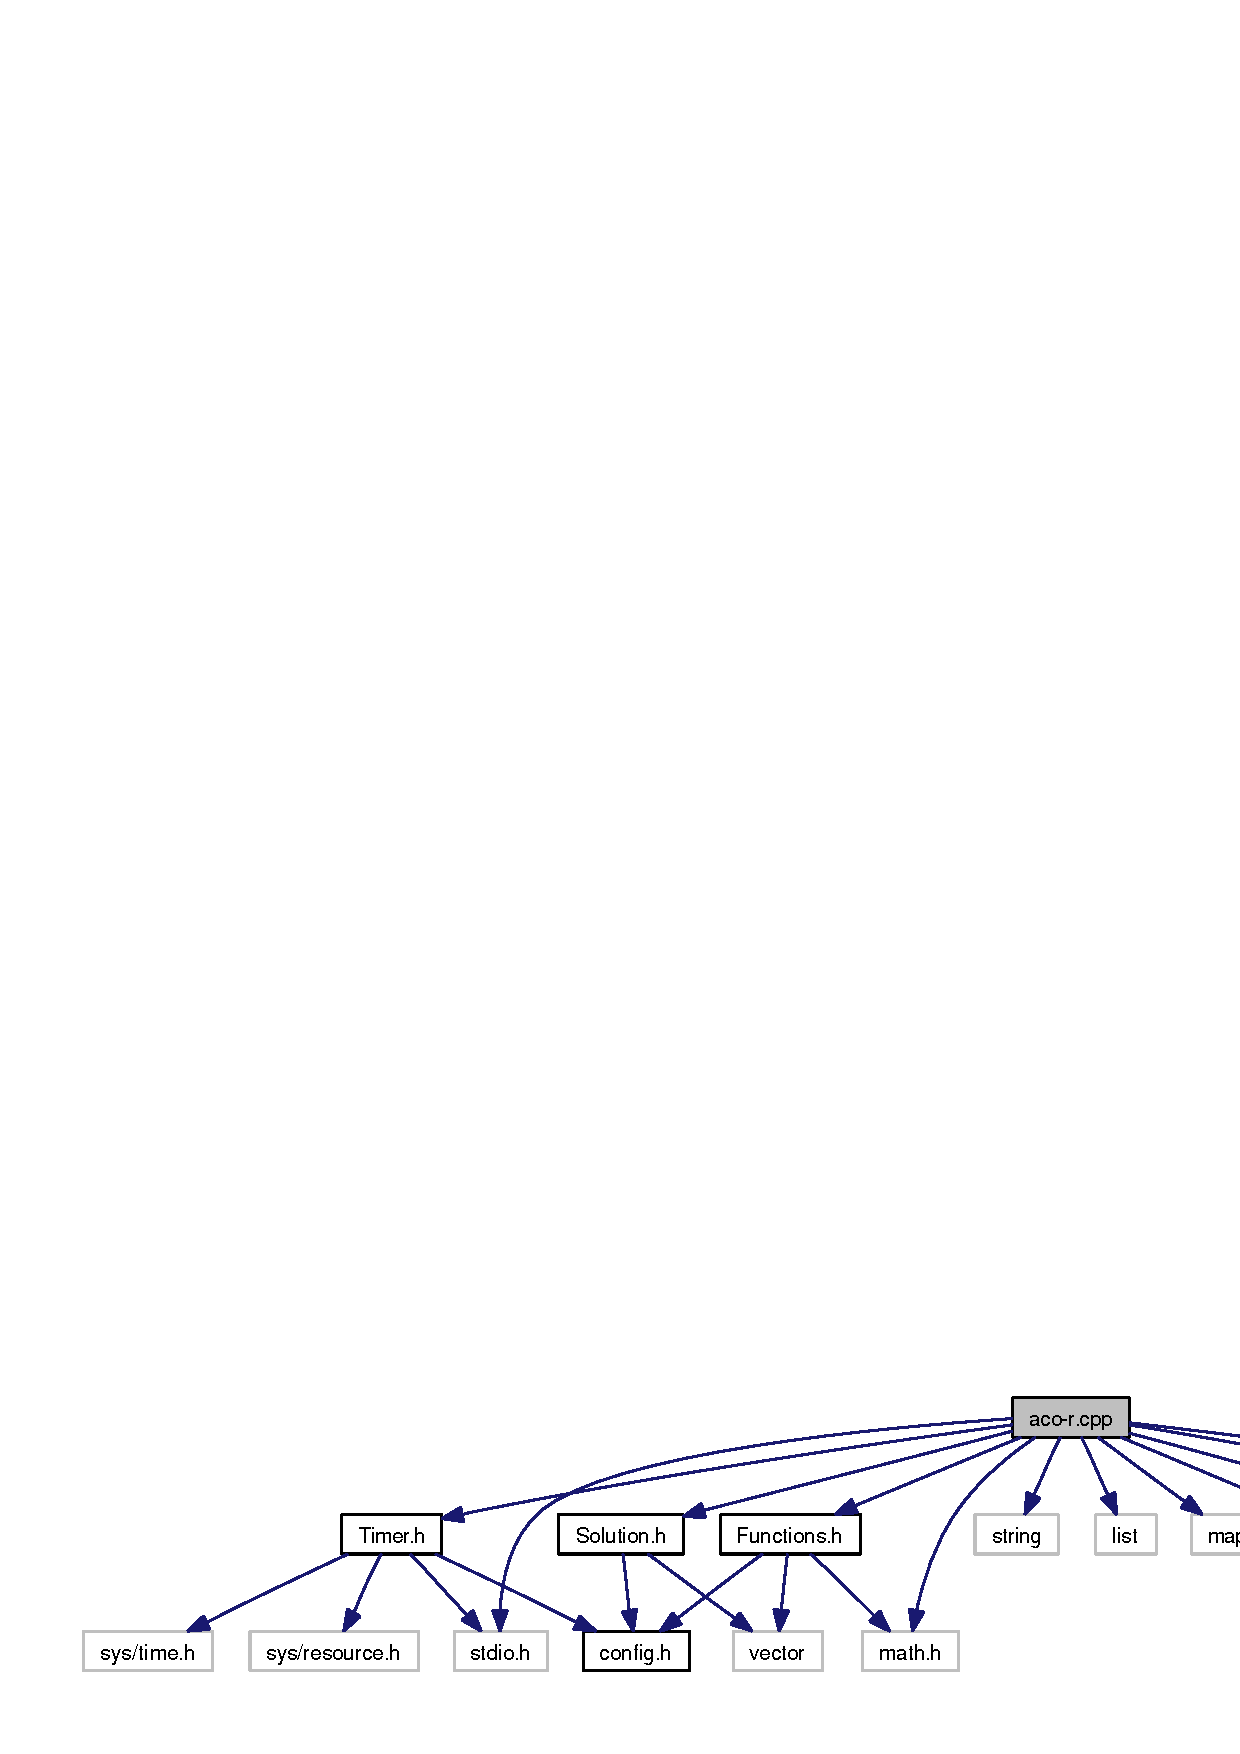
\includegraphics[width=420pt]{aco-r_8cpp__incl}
\end{center}
\end{figure}
\subsection*{Defines}
\begin{CompactItemize}
\item 
\#define \hyperlink{aco-r_8cpp_523b1c70fbff9e4e25f29b323bead209}{RAND\_\-UNIFORME}~(double)random()/(double)RAND\_\-MAX
\end{CompactItemize}
\subsection*{Functions}
\begin{CompactItemize}
\item 
void \hyperlink{aco-r_8cpp_02fd73d861ef2e4aabb38c0c9ff82947}{init} ()
\item 
double \hyperlink{aco-r_8cpp_c49c8f28940eb73a2d3c5d4f54a77acb}{gaussian} (double mean, double var)
\item 
void \hyperlink{aco-r_8cpp_cec77708e3d6f73a14c252e8747c11b1}{print\_\-best\_\-solution} (\hyperlink{classSolution}{Solution} bSol, \hyperlink{classFunction}{Function} $\ast$af, \hyperlink{classTimer}{Timer} \&atimer, int icount)
\item 
double \hyperlink{aco-r_8cpp_c5992296530c3f2c91fb35345606b029}{evaluate} (double $\ast$s)
\item 
int \hyperlink{aco-r_8cpp_3c04138a5bfe5d72780bb7e82a18e627}{main} (int argc, char $\ast$$\ast$argv)
\end{CompactItemize}
\subsection*{Variables}
\begin{CompactItemize}
\item 
double $\ast$ \hyperlink{aco-r_8cpp_a0e91b6673e0f6c62ed362a35d18064e}{archive} = NULL
\item 
double $\ast$ \hyperlink{aco-r_8cpp_68e32a83dbc9e45c0eca86384c297aba}{constrains} = NULL
\item 
int \hyperlink{aco-r_8cpp_1a8a8235879363159315091a1daed72f}{dimension} = 10
\item 
int \hyperlink{aco-r_8cpp_ae8c272782ff802dd95092adf15f474e}{archive\_\-size} = 5
\item 
int \hyperlink{aco-r_8cpp_346cfde20df32ef1244e37b7de85f5a3}{number\_\-of\_\-ants} = 3
\item 
int \hyperlink{aco-r_8cpp_77d5d27d8fdf89eb369e3bae9e6e752d}{number\_\-of\_\-iterations} = 100
\item 
double \hyperlink{aco-r_8cpp_5b5e3f03e443adea974601f295136638}{q} = 1.0
\item 
double \hyperlink{aco-r_8cpp_3ed57096651b587c2bf716fa78048153}{rho} = 1.0
\end{CompactItemize}


\subsection{Define Documentation}
\hypertarget{aco-r_8cpp_523b1c70fbff9e4e25f29b323bead209}{
\index{aco-r.cpp@{aco-r.cpp}!RAND\_\-UNIFORME@{RAND\_\-UNIFORME}}
\index{RAND\_\-UNIFORME@{RAND\_\-UNIFORME}!aco-r.cpp@{aco-r.cpp}}
\subsubsection{\setlength{\rightskip}{0pt plus 5cm}\#define RAND\_\-UNIFORME~(double)random()/(double)RAND\_\-MAX}}
\label{aco-r_8cpp_523b1c70fbff9e4e25f29b323bead209}




\subsection{Function Documentation}
\hypertarget{aco-r_8cpp_c5992296530c3f2c91fb35345606b029}{
\index{aco-r.cpp@{aco-r.cpp}!evaluate@{evaluate}}
\index{evaluate@{evaluate}!aco-r.cpp@{aco-r.cpp}}
\subsubsection{\setlength{\rightskip}{0pt plus 5cm}double evaluate (double $\ast$ {\em s})}}
\label{aco-r_8cpp_c5992296530c3f2c91fb35345606b029}


\hypertarget{aco-r_8cpp_c49c8f28940eb73a2d3c5d4f54a77acb}{
\index{aco-r.cpp@{aco-r.cpp}!gaussian@{gaussian}}
\index{gaussian@{gaussian}!aco-r.cpp@{aco-r.cpp}}
\subsubsection{\setlength{\rightskip}{0pt plus 5cm}double gaussian (double {\em mean}, \/  double {\em var})}}
\label{aco-r_8cpp_c49c8f28940eb73a2d3c5d4f54a77acb}


\hypertarget{aco-r_8cpp_02fd73d861ef2e4aabb38c0c9ff82947}{
\index{aco-r.cpp@{aco-r.cpp}!init@{init}}
\index{init@{init}!aco-r.cpp@{aco-r.cpp}}
\subsubsection{\setlength{\rightskip}{0pt plus 5cm}void init ()}}
\label{aco-r_8cpp_02fd73d861ef2e4aabb38c0c9ff82947}


\hypertarget{aco-r_8cpp_3c04138a5bfe5d72780bb7e82a18e627}{
\index{aco-r.cpp@{aco-r.cpp}!main@{main}}
\index{main@{main}!aco-r.cpp@{aco-r.cpp}}
\subsubsection{\setlength{\rightskip}{0pt plus 5cm}int main (int {\em argc}, \/  char $\ast$$\ast$ {\em argv})}}
\label{aco-r_8cpp_3c04138a5bfe5d72780bb7e82a18e627}




Here is the call graph for this function:\nopagebreak
\begin{figure}[H]
\begin{center}
\leavevmode
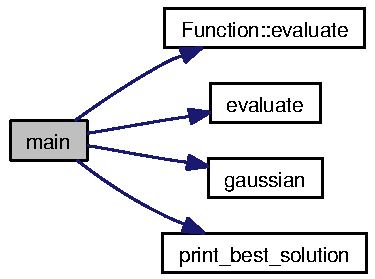
\includegraphics[width=108pt]{aco-r_8cpp_3c04138a5bfe5d72780bb7e82a18e627_cgraph}
\end{center}
\end{figure}
\hypertarget{aco-r_8cpp_cec77708e3d6f73a14c252e8747c11b1}{
\index{aco-r.cpp@{aco-r.cpp}!print\_\-best\_\-solution@{print\_\-best\_\-solution}}
\index{print\_\-best\_\-solution@{print\_\-best\_\-solution}!aco-r.cpp@{aco-r.cpp}}
\subsubsection{\setlength{\rightskip}{0pt plus 5cm}void print\_\-best\_\-solution ({\bf Solution} {\em bSol}, \/  {\bf Function} $\ast$ {\em af}, \/  {\bf Timer} \& {\em atimer}, \/  int {\em icount})}}
\label{aco-r_8cpp_cec77708e3d6f73a14c252e8747c11b1}




\subsection{Variable Documentation}
\hypertarget{aco-r_8cpp_a0e91b6673e0f6c62ed362a35d18064e}{
\index{aco-r.cpp@{aco-r.cpp}!archive@{archive}}
\index{archive@{archive}!aco-r.cpp@{aco-r.cpp}}
\subsubsection{\setlength{\rightskip}{0pt plus 5cm}double$\ast$ {\bf archive} = NULL}}
\label{aco-r_8cpp_a0e91b6673e0f6c62ed362a35d18064e}


\hypertarget{aco-r_8cpp_ae8c272782ff802dd95092adf15f474e}{
\index{aco-r.cpp@{aco-r.cpp}!archive\_\-size@{archive\_\-size}}
\index{archive\_\-size@{archive\_\-size}!aco-r.cpp@{aco-r.cpp}}
\subsubsection{\setlength{\rightskip}{0pt plus 5cm}int {\bf archive\_\-size} = 5}}
\label{aco-r_8cpp_ae8c272782ff802dd95092adf15f474e}


\hypertarget{aco-r_8cpp_68e32a83dbc9e45c0eca86384c297aba}{
\index{aco-r.cpp@{aco-r.cpp}!constrains@{constrains}}
\index{constrains@{constrains}!aco-r.cpp@{aco-r.cpp}}
\subsubsection{\setlength{\rightskip}{0pt plus 5cm}double$\ast$ {\bf constrains} = NULL}}
\label{aco-r_8cpp_68e32a83dbc9e45c0eca86384c297aba}


\hypertarget{aco-r_8cpp_1a8a8235879363159315091a1daed72f}{
\index{aco-r.cpp@{aco-r.cpp}!dimension@{dimension}}
\index{dimension@{dimension}!aco-r.cpp@{aco-r.cpp}}
\subsubsection{\setlength{\rightskip}{0pt plus 5cm}int {\bf dimension} = 10}}
\label{aco-r_8cpp_1a8a8235879363159315091a1daed72f}


\hypertarget{aco-r_8cpp_346cfde20df32ef1244e37b7de85f5a3}{
\index{aco-r.cpp@{aco-r.cpp}!number\_\-of\_\-ants@{number\_\-of\_\-ants}}
\index{number\_\-of\_\-ants@{number\_\-of\_\-ants}!aco-r.cpp@{aco-r.cpp}}
\subsubsection{\setlength{\rightskip}{0pt plus 5cm}int {\bf number\_\-of\_\-ants} = 3}}
\label{aco-r_8cpp_346cfde20df32ef1244e37b7de85f5a3}


\hypertarget{aco-r_8cpp_77d5d27d8fdf89eb369e3bae9e6e752d}{
\index{aco-r.cpp@{aco-r.cpp}!number\_\-of\_\-iterations@{number\_\-of\_\-iterations}}
\index{number\_\-of\_\-iterations@{number\_\-of\_\-iterations}!aco-r.cpp@{aco-r.cpp}}
\subsubsection{\setlength{\rightskip}{0pt plus 5cm}int {\bf number\_\-of\_\-iterations} = 100}}
\label{aco-r_8cpp_77d5d27d8fdf89eb369e3bae9e6e752d}


\hypertarget{aco-r_8cpp_5b5e3f03e443adea974601f295136638}{
\index{aco-r.cpp@{aco-r.cpp}!q@{q}}
\index{q@{q}!aco-r.cpp@{aco-r.cpp}}
\subsubsection{\setlength{\rightskip}{0pt plus 5cm}double {\bf q} = 1.0}}
\label{aco-r_8cpp_5b5e3f03e443adea974601f295136638}


\hypertarget{aco-r_8cpp_3ed57096651b587c2bf716fa78048153}{
\index{aco-r.cpp@{aco-r.cpp}!rho@{rho}}
\index{rho@{rho}!aco-r.cpp@{aco-r.cpp}}
\subsubsection{\setlength{\rightskip}{0pt plus 5cm}double {\bf rho} = 1.0}}
\label{aco-r_8cpp_3ed57096651b587c2bf716fa78048153}


